\section{Conclusion}
%!TEX root = prelim.tex
%!TEX root = fakeroot.tex



%To date, I have performed two experiments have been performed to guide the choice of training illuminations, the results of which were shown in Chapter \ref{chap:cvpr}.  One used rectangular partitions of the domain of the illumination space with different granularities.  This gave a rough idea of the number of training illuminations that would be necessary.  The second experiment used a partitions of the illumination domain that were rectangular in a polar coordinate system.  This gave a rough idea of the range of angles the training images should cover.  Our large training database was acquired by combining these two pieces of information.  While a study of the choice of training illuminations at this granularity is already unprecedented for face recognition, \footnote{ Several studies, including \cite{Basri2003-PAMI, LeeK2005-PAMI} have used images rendered from a 3D face model to optimize their choice of illumination.  Similar illumination studies have also been performed on other objects for graphics applications.} only a very small subset of the possible illuminations was explored compared to what the projectors are capable of.  For instance, how many of the frontal images are necessary?  Should some directions receive a higher density of illuminations than others? 

%\subsection{Optimize illuminations within the set of training images we already have}
%One option we have for optimizing our training illuminations is to use the training and testing databases we have already gathered, and to search for a lower dimensional subspace of illuminations that still has a good recognition rate.  The two main advantages of this strategy are that the recognition rate can be computed directly and used as a measure of the quality of the training images, and that the sizable database we have already gathered can be used.  The main disadvantage is that we will most likely have to trade some accuracy for speed, since we can only restrict the number of measurements the algorithm uses. \footnote{It could be possible for a subset of the illuminations is more discriminating than the full set; however this would be a very surprising result indeed!}

%\subsection{Optimize illuminations with the illumination system in the loop}
%A second option is to perform an optimization of the training image space with the image acquisition system in the loop.  The main advantage is that we can include any training images we want to in the optimizaztion.  The main disadvantage is that we cannot compute a recognition rate and instead have to resort to using representation error as a measure of the quality of the training images.  Why can't we just capture and store a the images generated by a complete basis for the space of illuminations, and then optimize over weighted combinations of them?  If a single projector pixel is illuminated at a time, it would take over 4 TB of data to store the remaining images, and take 28 hours to capture; this wouldn't be convenient, but it could be managed.  Unfortunately, there is a problem with this idea:  in every image you take, the actual signal would fall below the noise floor of the camera.  For this reason it is critical to capture images with a significant portion of the projector pixels illuminated at a time.  Keeping the real world in the loop solves this problem without resorting to arbitrarily enforcing a minimum block size.  Due to the extremely long time that the subject will have to remain motionless while the optimization runs, a movie-grade dummy head would be a good candidate for the training subject.  

%This still leaves several interesting questions.  Even with an automated search, we are going to have to make some assumptions to reduce the search space.  Should we allow for pixels to be partially turned on, or should they be binary?  Should we require illuminations to have pixels that are all adjacent?  What metric should we use to measure the quality of the training images?  Ideally we'd be using a large database of real subjects, but that is not an option if we want to search over the full set of illuminations the projectors can generate.  How many training images should we allow?  How do we quantify the tradeoff between speed and accuracy?

%There are few other things that make this experiment appealing.  Since the dummy head is inanimate, we will completely eliminate the influence of pose variation on the experiment, and all of our training images will already be perfectly aligned; the cameras can be manually positioned such that the frontal and rear illuminations match up perfectly. \footnote{Since we want to capture training illuminations from both sides, the dummy head can be mounted on a stepper-motor driven pivot for the purpose of rotating the dummy head by 180 degrees.  }

%\subsection{Leverage color information to improve occlusion robustness}  Color information is unused for the current system.  This was a simplifying assumption that made implementation of the algorithm significantly easier and faster.  There are several different ways in which the algorithms presented in this thesis could be extended to handle color information.  One of the main reasons that color is not as important in face recognition as it is in some other vision applications is that the pixels in the image of a given person's face generally vary primarily in intensity.  Furthermore, the variation of skin tone from person to person usually varies less than the color variation resulting from the color of the illumination.  For these reasons, color may be especially useful for the improvement of occlusion handling, since occluding objects are likely to vary in color more than human faces do.  




%\frame{
%\frametitle{Loading the training database}
%\begin{itemize}
%\item
%\item
%\item
%\end{itemize}
%}

%\subsection{Optimizing the Speed of the Recognition Algorithm}
%\frame{\tableofcontents[currentsection, currentsubsection]}

%\frame{
%\frametitle{Loading the training database}
%\begin{center}
%%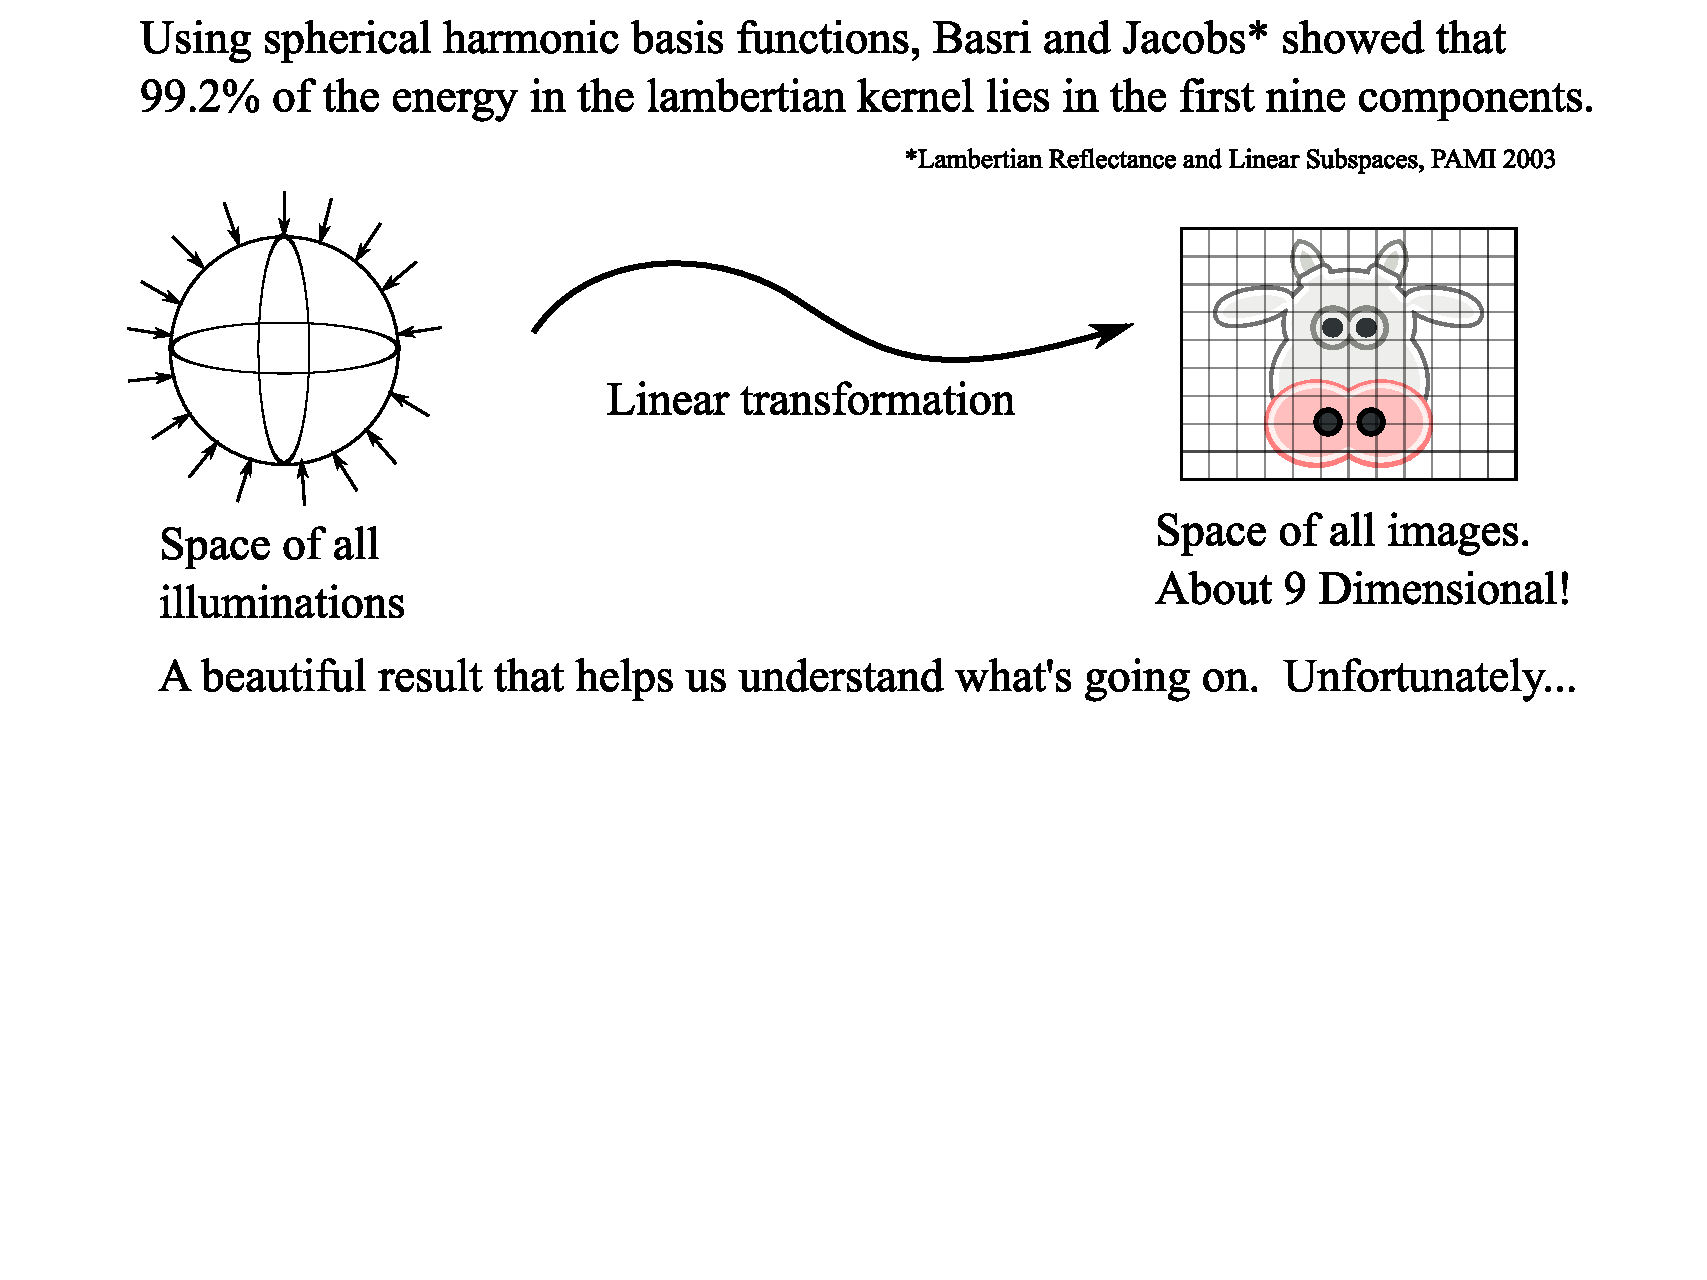
\includegraphics[width=0.8\textwidth]{images/basri3.pdf}
%\end{center}
%}

%\frame{
%\frametitle{Per-user alignment}
%\begin{center}
%%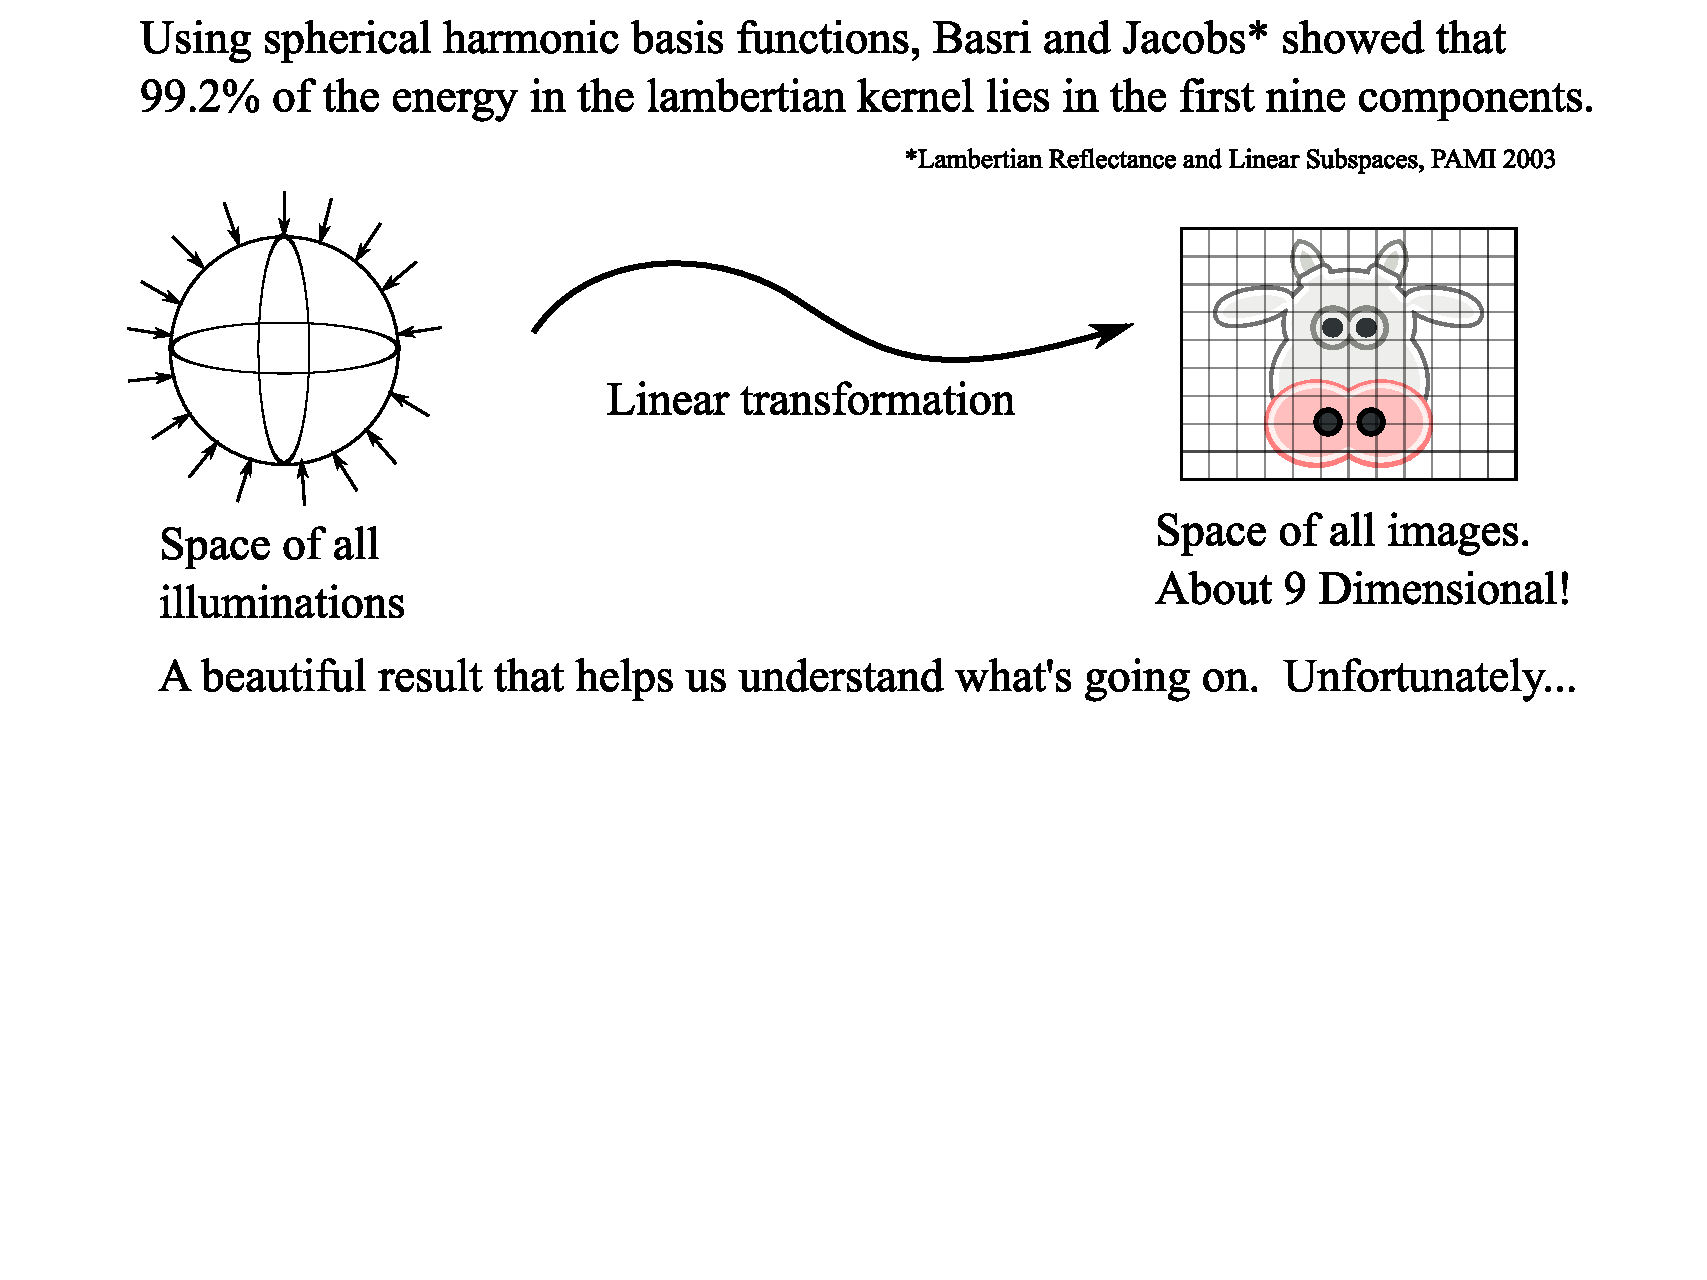
\includegraphics[width=0.8\textwidth]{images/basri3.pdf}
%\end{center}
%}

%\frame{
%\frametitle{Resampling the training images}
%\begin{center}
%%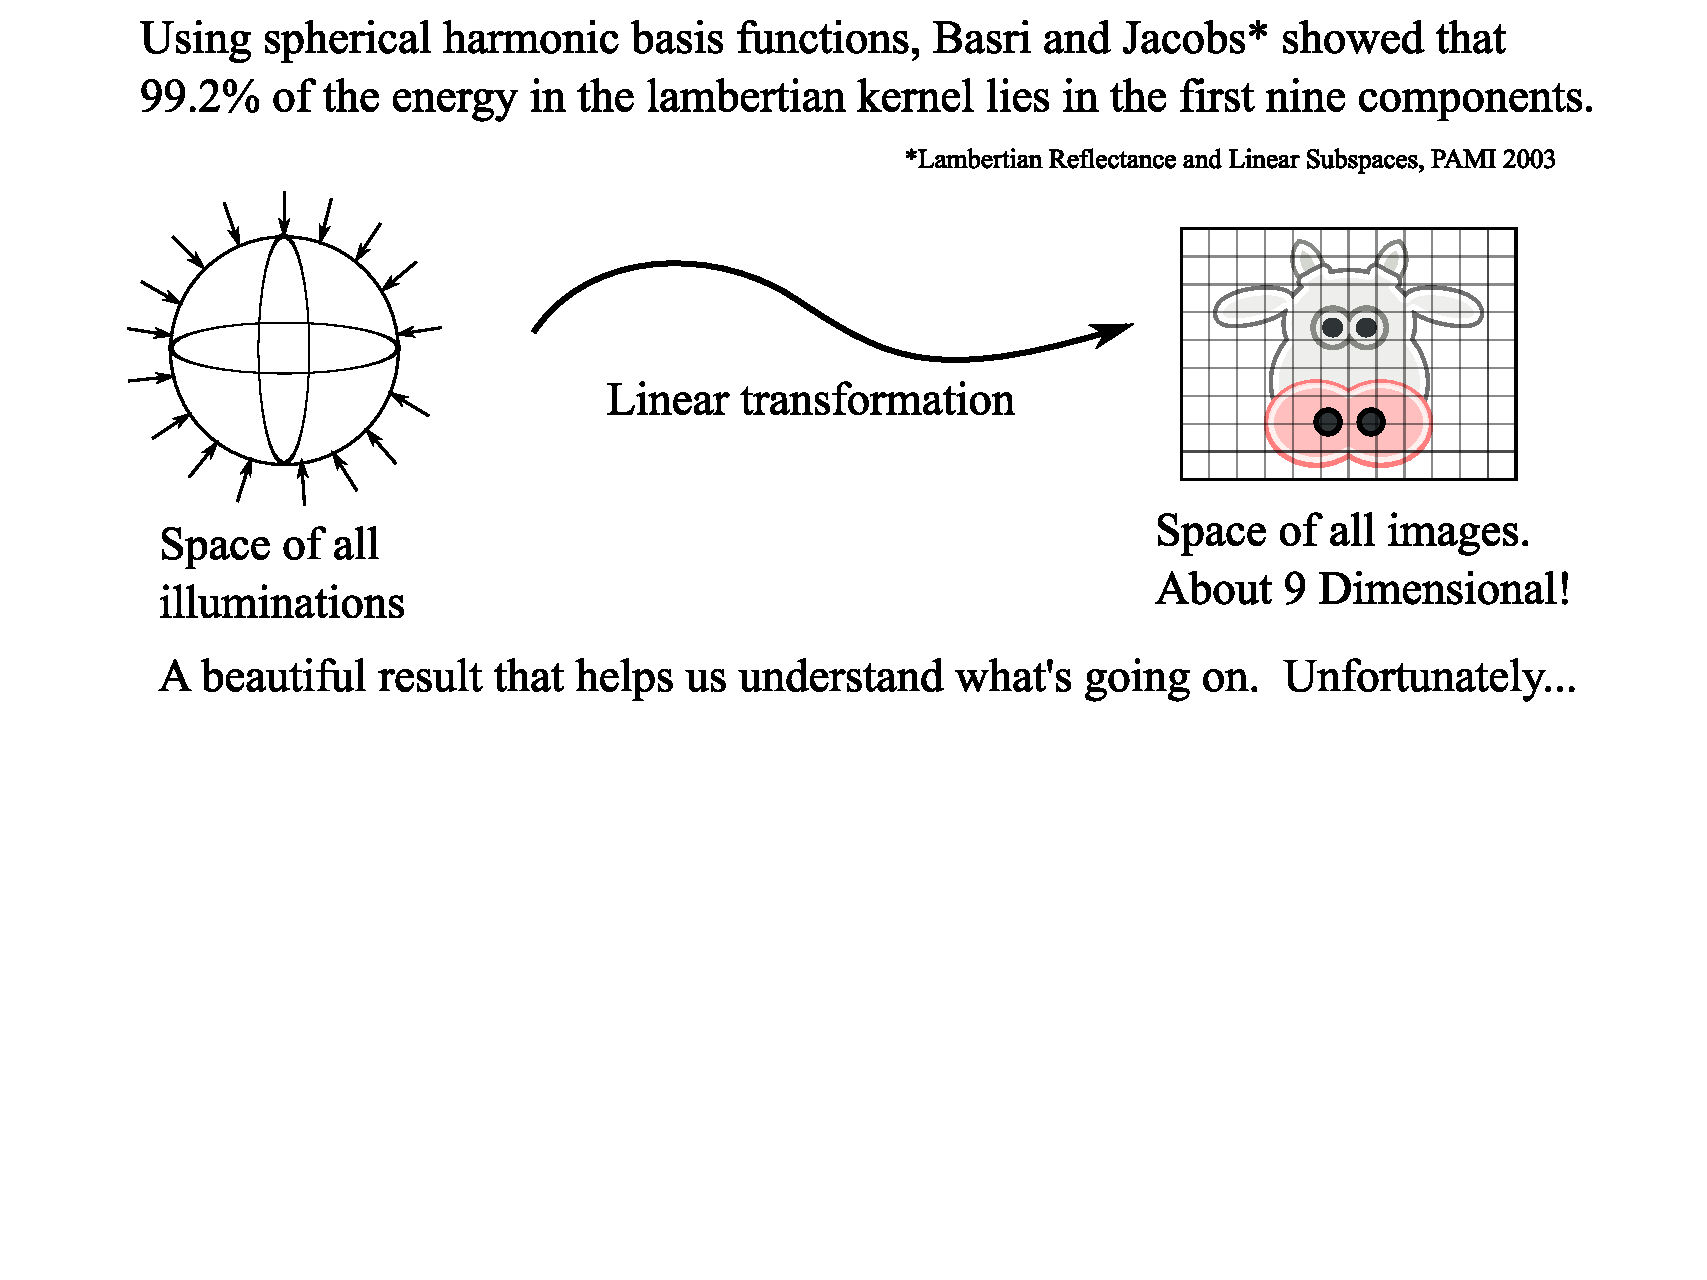
\includegraphics[width=0.8\textwidth]{images/basri3.pdf}
%\end{center}
%}

%\frame{
%\frametitle{Final recognition step}
%\begin{center}
%%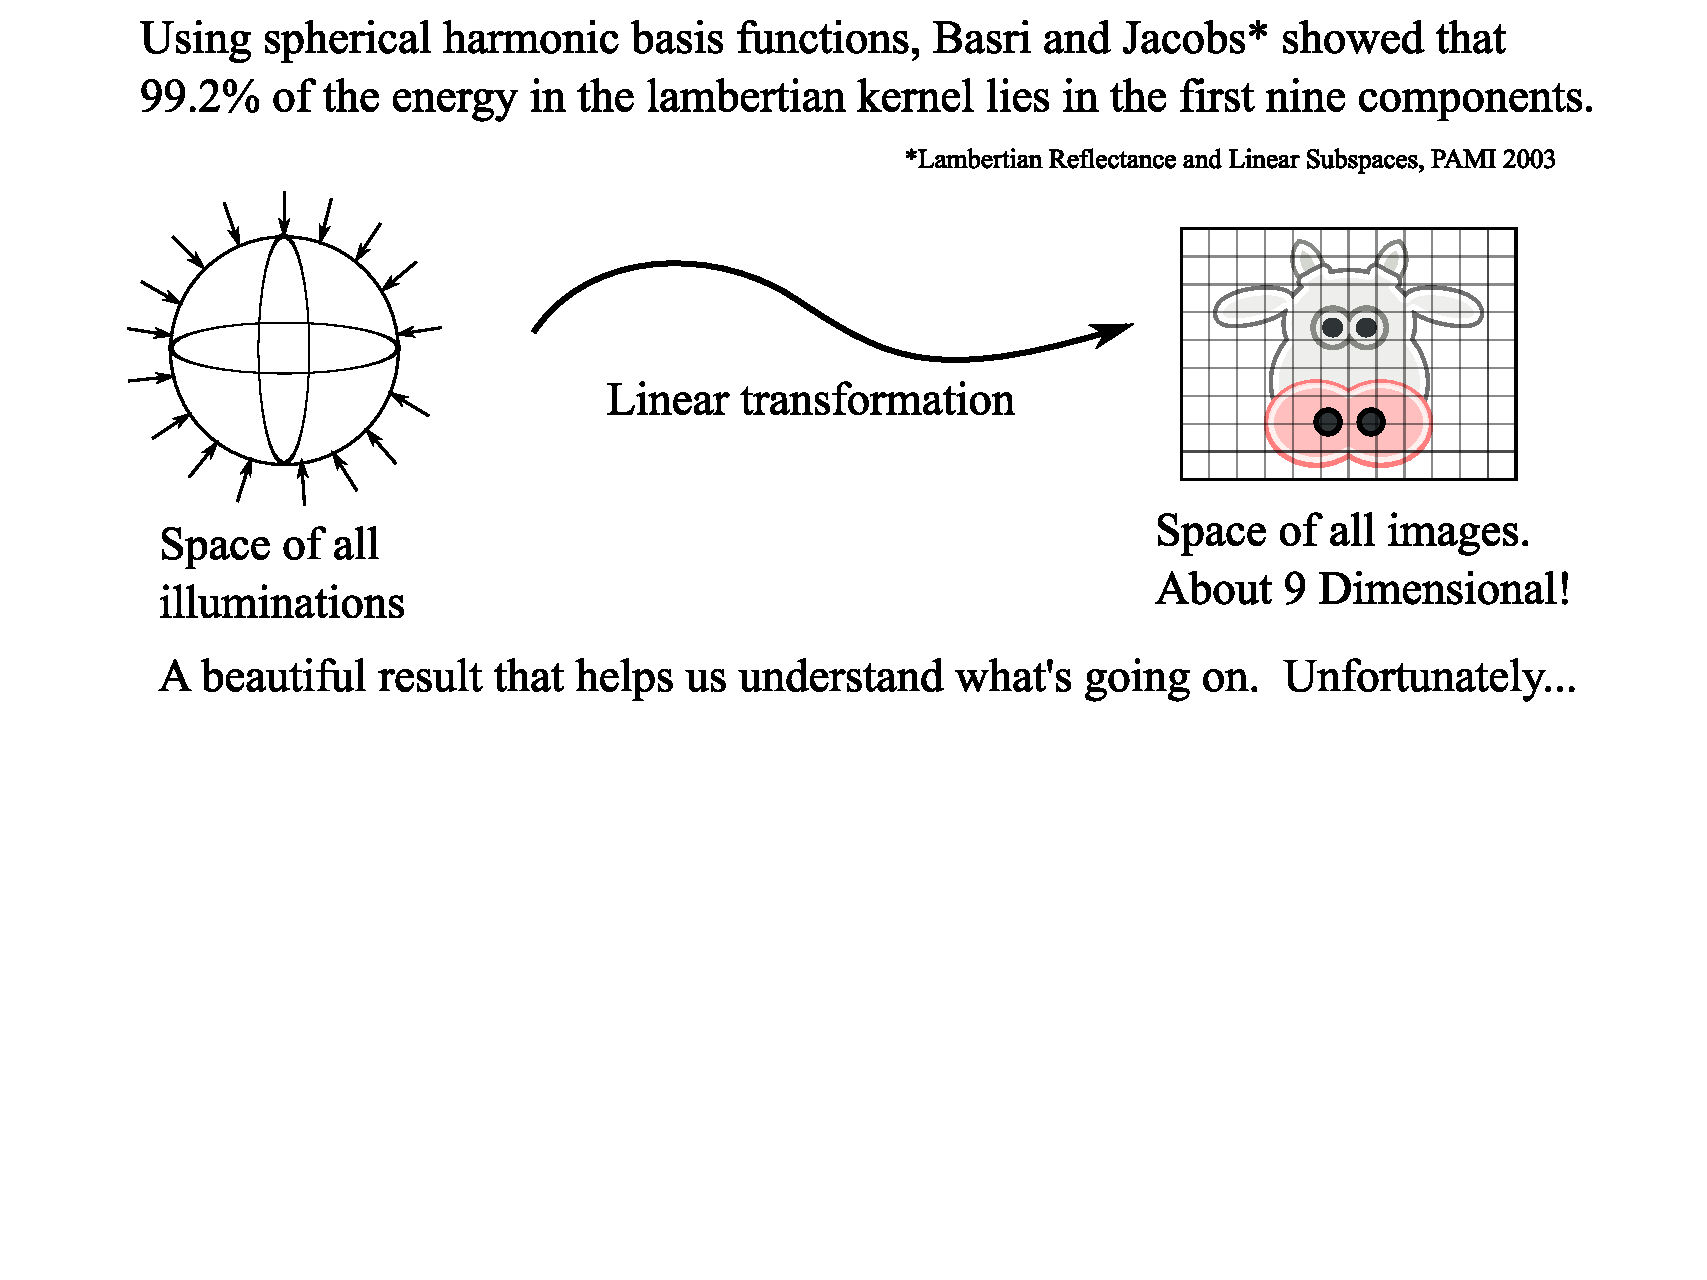
\includegraphics[width=0.8\textwidth]{images/basri3.pdf}
%\end{center}
%}

%\subsection{Optimizing the training illuminations}
%\frame{
%\frametitle{Optimize illuminations within the set of training images we already have}
%\begin{center}
%%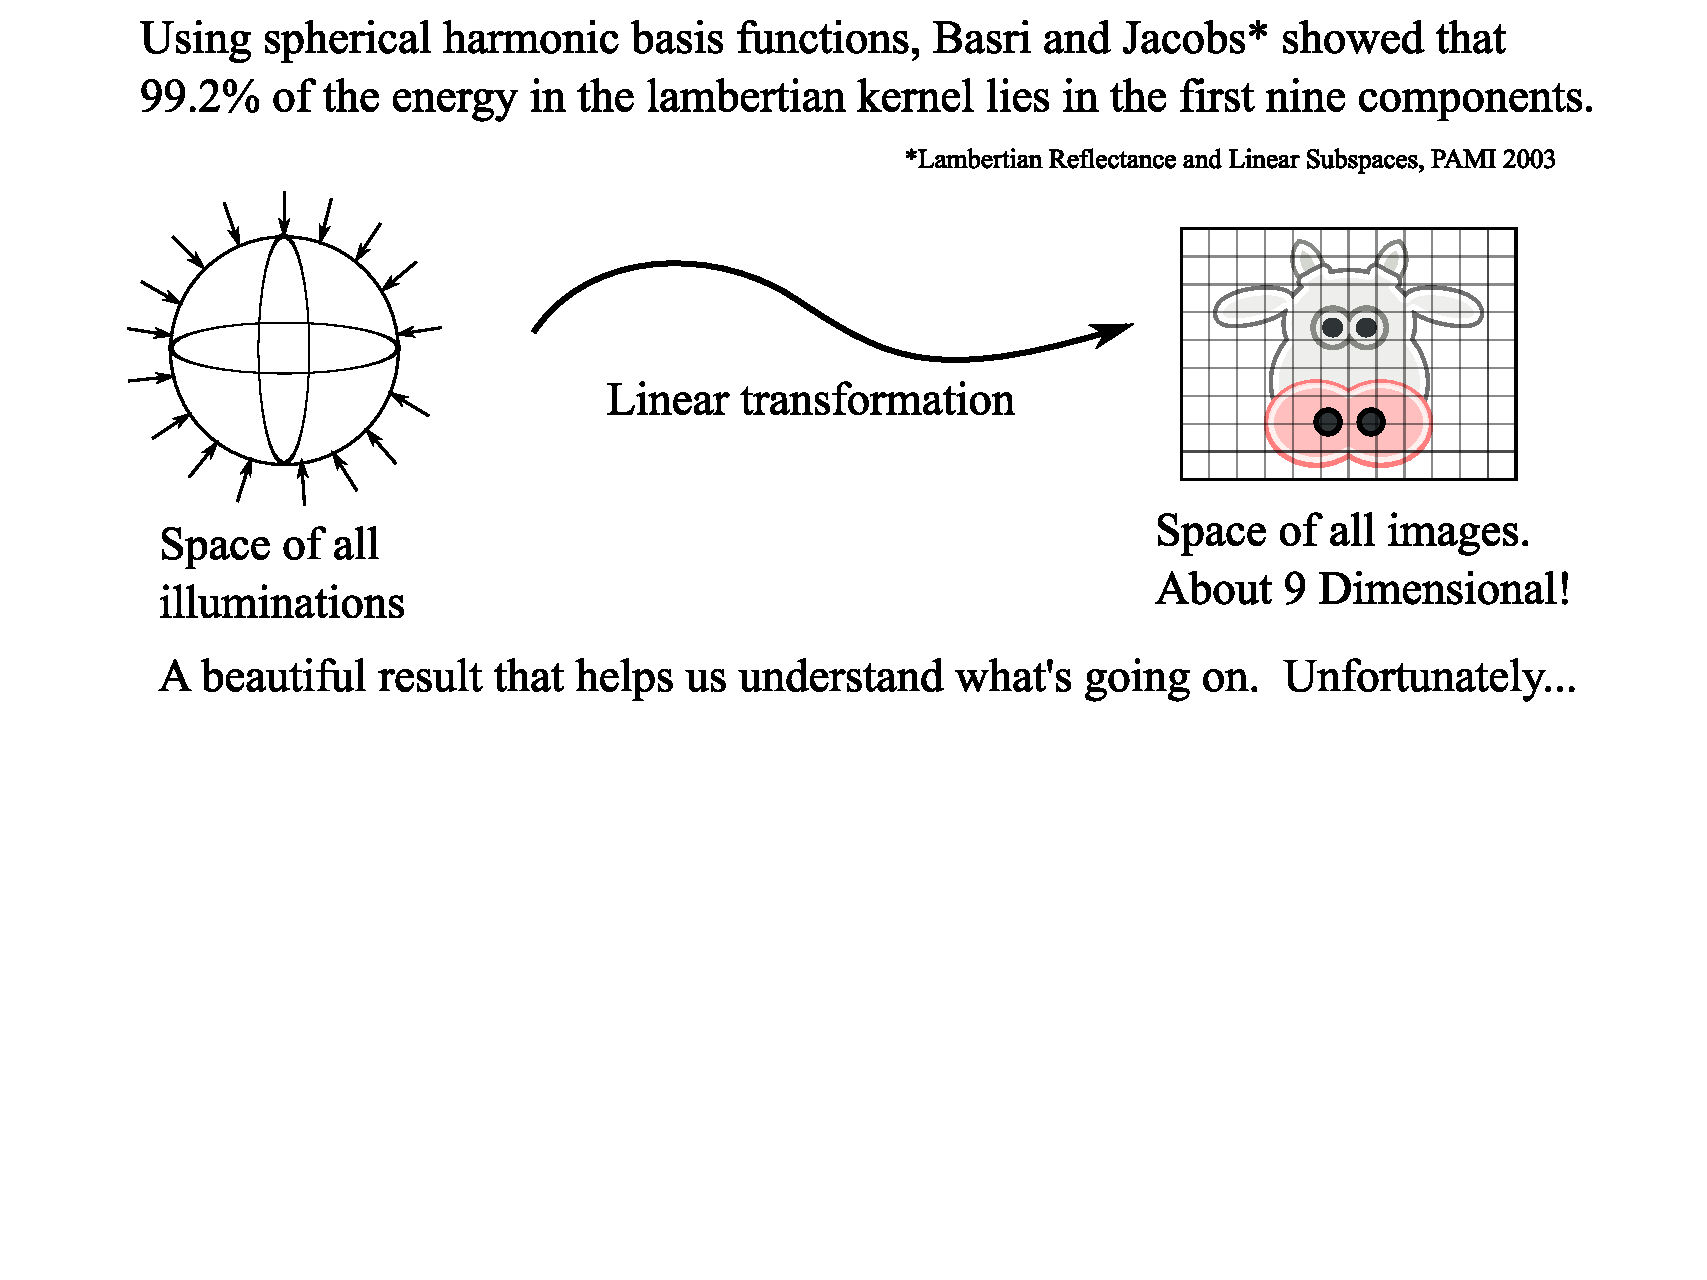
\includegraphics[width=0.8\textwidth]{images/basri3.pdf}
%\end{center}
%}

%\frame{
%\frametitle{Optimize illuminations with the illumination system in the loop}
%\begin{center}
%%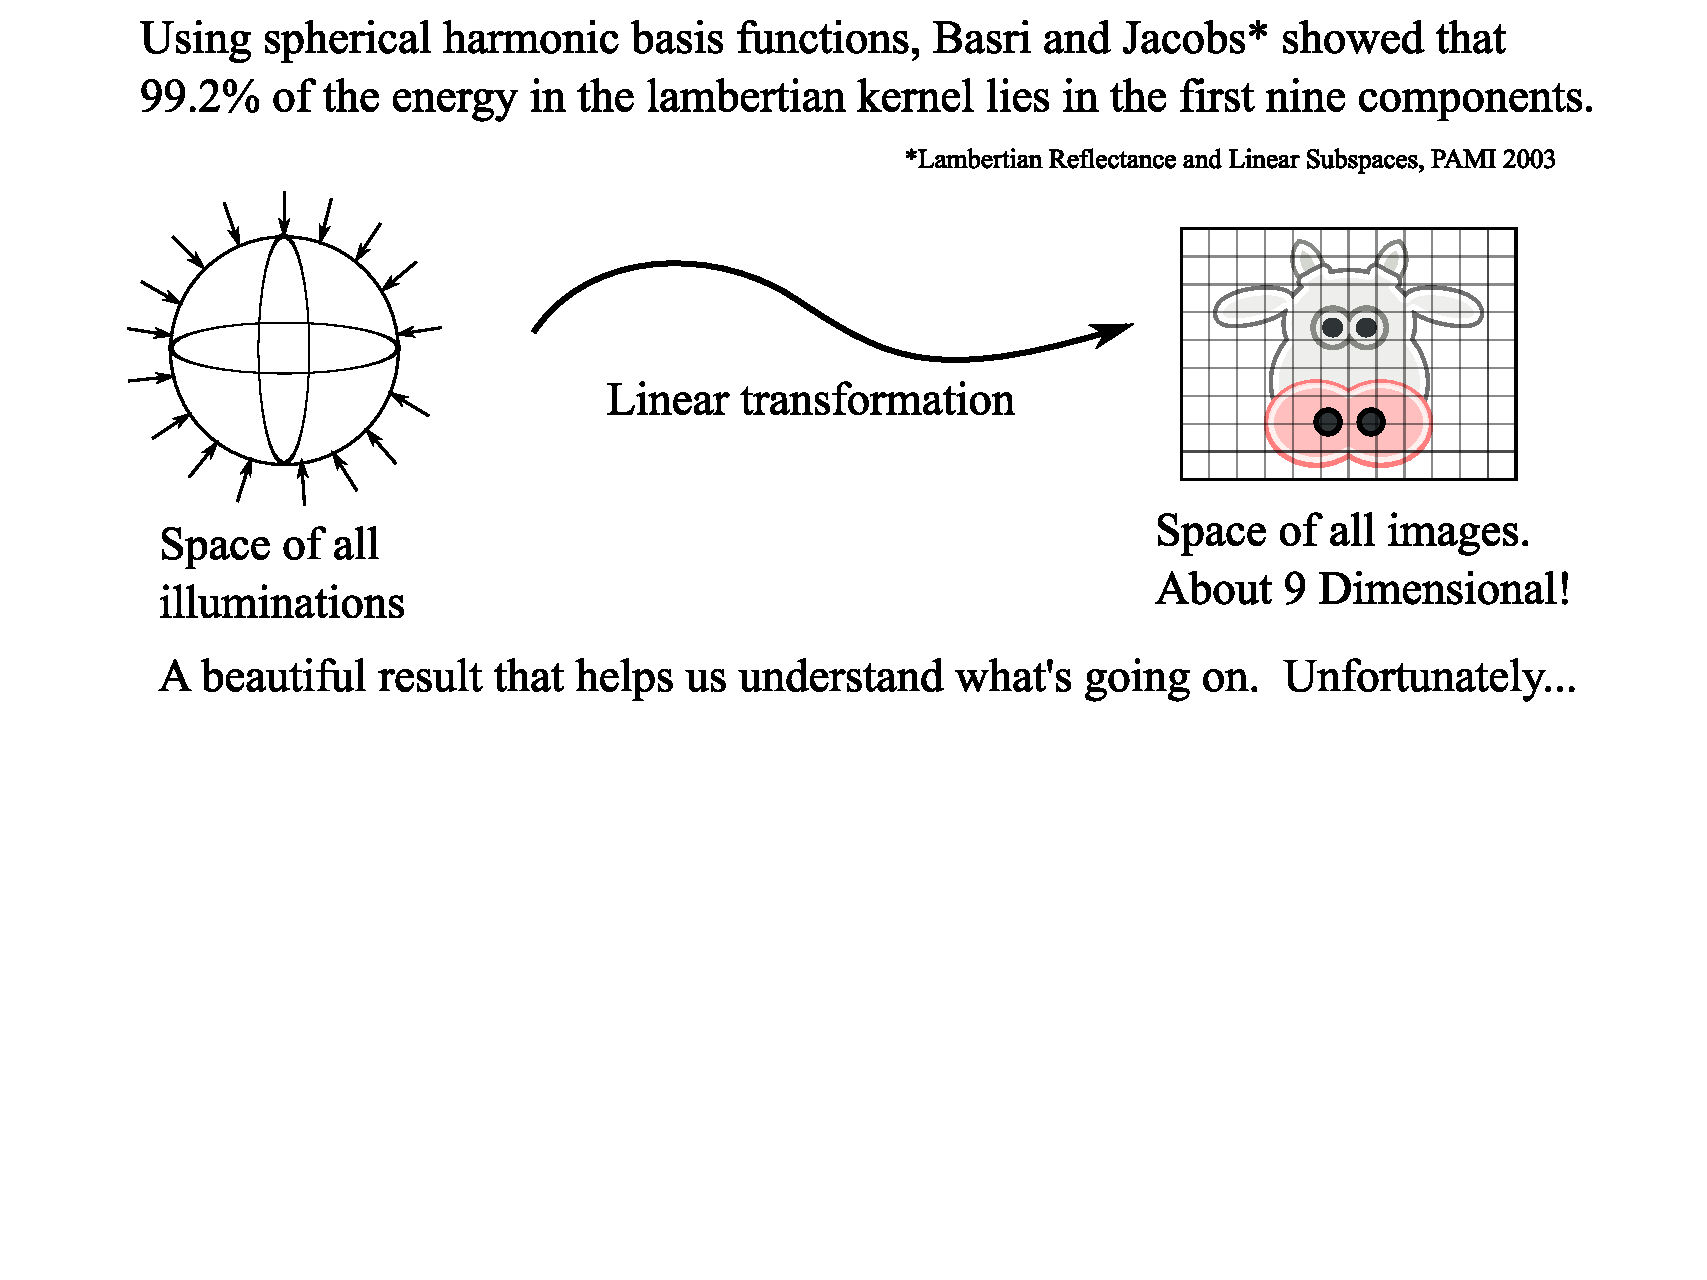
\includegraphics[width=0.8\textwidth]{images/basri3.pdf}
%\end{center}
%}
